\documentclass%
%% versión borrador (o corrector) -> descomentar la siguiente linea
%[borrador]%
{formats/tesisCNA}
%% Si no se quiere dedicar la tesis OPCIONAL -> descomentar la siguiente linea
%\def\nodedicatoria{1}
%% Si se va a hacer un índice alfabético (hay que ejecutar makeindex antes de lualatex !!), comentar la siguiente linea
\def\noindicealfabetico{1}
%% Si se quiere que aparezca la lista de figuras/tablas -> descomentar la siguiente linea
%\def\listatablasfiguras{1}%

% Equal in distribution
\newcommand{\eqdistr}{\,{\buildrel d \over =}\,}
\usepackage{hyperref}

\begin{document}
%% epígrafe OPCIONAL -> si no se desea, comentar la siguiente linea
\epigrafe
%%%% ¡¡¡ NO TOCAR LA SIGUIENTE LINEA !!!
\materialfijoinicial
% prólogo / preface OPCIONAL -> si no se desea, comentar la siguiente linea
\prefacio
% abreviaturas y símbolos / glossary OPCIONAL -> si no se desea, comentar la siguiente linea
\glosario
%%%% ¡¡¡ NO TOCAR LA SIGUIENTE LINEA !!!
\pagenumbering{arabic}%
%

%%%%%%%%%%%%%%%%%%%%%%%%%%%%%%%%%%%%%%%%%%%%%%%%%%%

\chapter{Introduction}
\label{chap:intro}

         % Introduction
\chapter{Market Risk}
\label{chap:MarketRisk}

\section{Market Risk}



\section{Market Risk Metrics}

\section{The Computational Burden of Market Risk Computations}

\section{Market Risk as a Supervised Machine Learning Problem} {\label{sec:MktRisk_SML}}

\section{Model Scores for Market Risk}

\section{Unsupervised Machine Learning Alternatives}
\subsection{Deep Learning}
\subsection{Differential Deep Learning}
\subsection{Other}

\newpage

\section{A Base Case Example}

As a base case example we consider an option for which a closed form solution exists. This allows us compare the results obtained by a supervised machine learning algorithm to those obtained by the closed form formula.

In order to add both non linear features and the possibility of increasing the dimension of the problem, we will use a call option on the geometric mean of a basket.

\begin{equation}\label{eq:geom_digital}
\begin{aligned}
&V_{T}=\max\left(G_T-k,0\right) \\
&G_{T}=\left(\prod_{j=1}^{m} \frac{S_{T}^{j}}{S_{0}^{j}}\right)^{1 / m} \\
\end{aligned}
\end{equation}

Where $S_t^1,\ldots,S_t^m$ represent the prices of the underlying assets as of time t and $G_T$ represents the geometric mean of one plus the return of the different assets from time $0$ to time $T$. $T$ represents the option's payoff date.

We assume geometric Brownian motion dynamics for the different underlying assets under the risk neutral measure:

\begin{equation}\label{eq:geom_brownianmotion}
\frac{S_{T}^{j}}{S_{t}^{j}}=\exp\left(\left(r-q_{j}-\frac{\sigma_{j}^{2}}{2}\right) \left( T - t\right)+\sigma_{j} \left(W_{T}^{j}-W_{t}^{j}\right)\right)
\end{equation}

Where $r$ represents the risk free rate, $q_j$ the continuous dividend yield , $\sigma_j$ the volatility and $W_T^j$ the change experienced form $0$ to $T$ of a Brownian motion. The $j$ index help us distinguish the parameters of the different underlying assets.

Taking into account \ref{eq:geom_brownianmotion}

\begin{equation}\label{eq:geom_digital_distrib}
\left(\prod_{j=1}^m\frac{S_{T}^{j}}{S_{0}^{j}}\right)^{\frac{1}{m}} =\left(\prod_{j=1}^m\frac{S_{t}^{j}}{S_{0}^{j}}\right)^{\frac{1}{m}}\exp\left(\frac{1}{m} \sum_{j=1}^{m}\left(r-q_{j}-\frac{\sigma_{j}^{2}}{2}\right) \left(T-t\right)+\frac{1}{m} \sum_{j=1}^{m} \sigma_{j} \left(W_{T}^{j}-W_{t}^{j}\right)\right) 
\end{equation}

Notice that $G_T$, conditional on $S_t^1,\cdots,S_t^m$ is log-normally distributed with parameters:



\begin{equation} 
\label{eq:geom_digital_distrib_params1}
\begin{aligned} 
& G_T|\mathcal{F}_t \eqdistr A \exp\left(\mu+\Sigma\phi\right)\\
& A = \left(\prod_{j=1}^m\frac{S_{t}^{j}}{S_{0}^{j}}\right)^{\frac{1}{m}} \\
&\mu = \frac{1}{m}\sum_{j=1}^{m}\left(r-q_{j}-\frac{\sigma_{j}^{2}}{2}\right)T \\   
& \Sigma=\frac{1}{m}\sqrt{\sigma^{\top} C_{w} \sigma}
\end{aligned}
\end{equation}

Where $\eqdistr$ represents equal in distribution, $\mathcal{F}_t$ the market filtration as of time $t$, $\sigma$ is a column vector containing the volatilities of the different underlying assets, $C_W$ the covariance matrix of $W_T^1,\cdots,W_T^m$ and $\phi$ is a standard normal distributed random variable.

\begin{equation} \label{eq:geom_digital_distrib_params2}
\begin{aligned}
&\sigma=\left[\begin{array}{c}
\sigma_{1} \\
\vdots \\
\sigma_{m}
\end{array}\right] \\
&C_{w}=\left[\begin{array}{cccc}
\left(T-t\right) & \rho_{12} \left(T-t\right) & \cdots & \rho_{1 m} \left(T-t\right) \\
\vdots & \vdots & & \vdots \\
\rho_{m 1} \left(T-t\right) & \rho_{m 2} \left(T-t\right) & \cdots &  \left(T-t\right)
\end{array}\right]
\end{aligned}
\end{equation} 

$\rho_{ij}$ represents the correlation of $W_t^i$ and $W_t^j$.

Given the distribution of $G_T$, the pricing formula as of time $t<T$ will be given by:

$$
\begin{array}{lll}
V_{t}&=&\exp (-r(T-t)) E_{\mathbb{Q}}\left[1_{\{G_{T}>K\}} | \mathcal{F}_t\right] \\
&& \\
&=&\left(A\exp\left(\mu+\frac{\Sigma^2}{2}\right)N\left(d_1\right)-k\left(d_2\right)\right)\exp\left(-r(T-t)\right)
\end{array}
$$

$$
\begin{aligned}
d_1 = \frac{\log\frac{A\exp\left(\mu+\frac{\Sigma^2}{2}\right)}{K}+\frac{\Sigma^2}{2}}{\Sigma} \\
d_2 = \frac{\log\frac{A\exp\left(\mu+\frac{\Sigma^2}{2}\right)}{K}-\frac{\Sigma^2}{2}}{\Sigma} \\
\end{aligned}
$$


% $$
% & E_{\mathbb{Q}}\left[1_{\{G_{T}>K\}} | \mathcal{F}_t\right]=P\left[Ae^{\mu+\sum \phi}>k\right] \\
% & =P\left[\phi<\frac{\log \frac{A}{K}+\mu}{\Sigma}\right]=N\left(\frac{\log \frac{A}{K}+\mu}{\Sigma}\right)
% \end{aligned}
% $$

Where $\phi$ represents a standard normal random variable and $N$ its cumulative distribution function. $\mathbb{Q}$ represents the risk neutral measure.


\subsection{Unhedged Portfolio}
 In this section we explore how the usage of machine learning techniques performs while trying to represent the payoff function in isolation. Nevertheless, we should keep in mind that it is common to perform market risk calculations for trading portfolios where exotics payoffs as the one introduced in the last section are hedged with vanilla instruments. This is the reason why in the next section we tackle the hedged portfolio case. 
 
 As payoff function we consider a call option on the geometric mean of a basket with two underlying assets $\{A,B\}$ with the following contract terms:
 
 \luis{Include more underlyings}
 
 \jorge{Test Jorge}
 
 \johan{Test Johan}
 
\begin{center}
\begin{tabular}{||c | c||} 
 \hline
 Market risk horizon $(\Delta)$ & $10$ days \\ 
 \hline
 Time to maturity $(T-t-\Delta)$ & $3$ years \\
 \hline
 $S_0^A$ & $1.0$ \\
 \hline
 $S_0^B$ & $1.0$ \\
 \hline
 $K$ & $1.0$ \\
 \hline
 \end{tabular}
\end{center}

We assume the following values for market variables (model parameters) as the market risk base scenario:

\begin{center}
\begin{tabular}{||c | c||} 
 \hline
 $S_t^A$ & 1.0 \\
 \hline
 $S_t^B$ & 1.0 \\
 \hline
 $\sigma_t^A$ & $0.2$ \\
 \hline
 $\sigma_t^B$ & $0.3$ \\
 \hline
 $r$ & $0.01$ \\
 \hline
 $q_A$ & $0.0$ \\
 \hline
 $q_B$ & $0.0$ \\
 \hline
 $rho$ & $0.8$ \\
 \hline
\end{tabular}
\end{center}

We apply market risk scenarios to $S_t^A,\ S_t^B,\ \sigma_t^A,\ \sigma_t^B$.
In order to apply market risk scenarios we make use of historical data for both the spot prices and the $1$ year implied at the money volatilities of BBVA and Santander from 2019-11-12 to 2021-10-11 (500 scenarios) \footnote{Source: Bloomberg}. We compute $10$ days log-normal overlapping returns from the historical data and apply these to our market risk variables $S_t^A,\ S_t^B,\ \sigma_t^A,\ \sigma_t^B$.

\luis{Use US stocks instead? Johan opinion?}

In the following figure we represent the $10$ days overlapping log returns of our historical data:

\begin{figure}[h] 
\centering
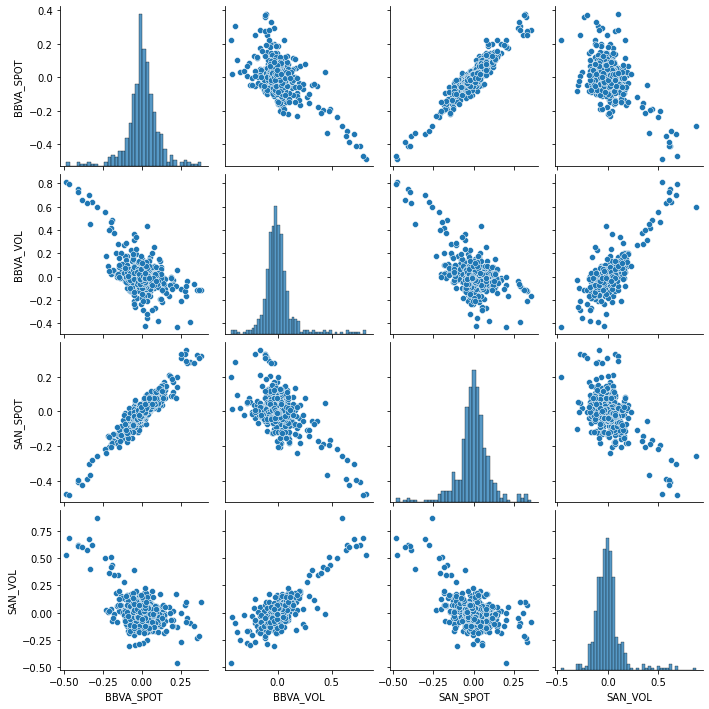
\includegraphics[width=0.7\textwidth]{Figures/MarketRisk/histdata.png}
\caption{Distribution of $10$ days log returns of market data. Marginal distributions of the different risk factors are plotted in the diagonal. Pairwise joint distributions are plotted in off diagonal figures.}
\label{fig:distrib_P}
\end{figure}

As we described in section \ref{sec:MktRisk_SML}, in order to train our supervised machine learning model, we generate synthetic data distributed as the data in Figure \ref{fig:distrib_P}. We sample $100000$ scenarios to train our models and $20000$ to cross-validate them. In order to do so, we  fit a Gaussian Mixture model to the data using the implementation in \href{https://scikit-learn.org/stable/modules/generated/sklearn.mixture.GaussianMixture.html}{Scikit Learn} with 5 components. The generation of synthetic data will be tackled in chapter \ref{chap:Synthetic}.

\luis{Comment a little bit more on why using the Gaussian Mixture}

\begin{figure}[h] 
\centering
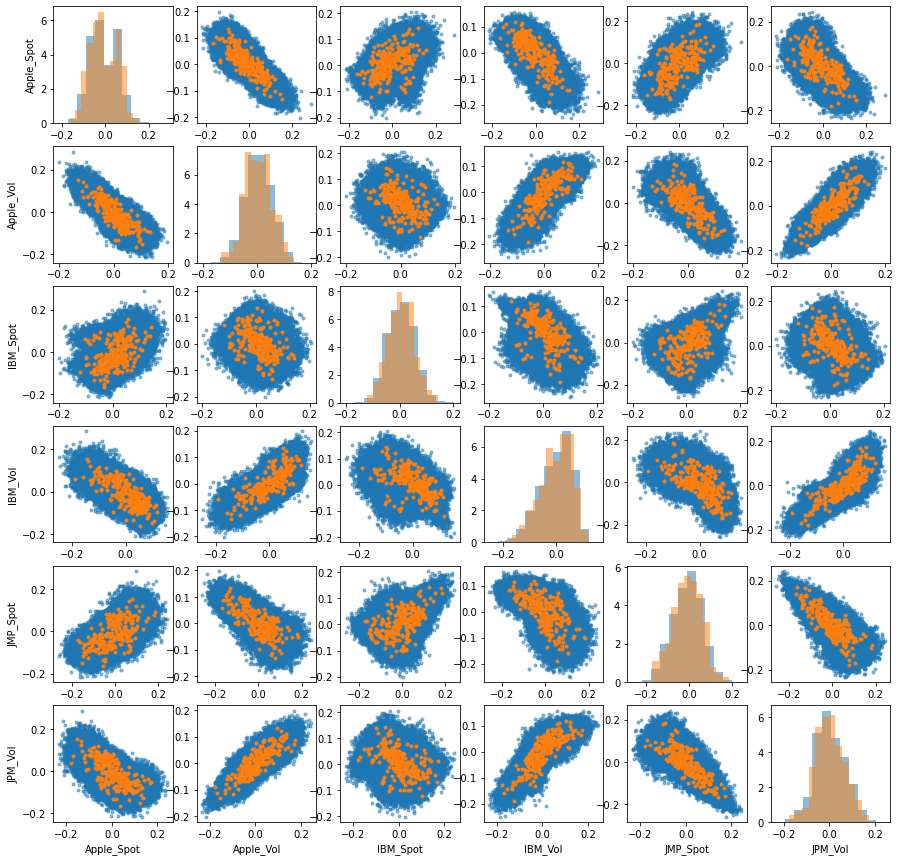
\includegraphics[width=0.7\textwidth]{Figures/MarketRisk/GaussMixture.png}
\caption{}
\label{fig:distrib_P}
\end{figure}

For each of these scenarios generated under the historical measure $\mathbb{P}$ that take us from $t$ (base scenario date) to $t+\Delta$, with $\Delta$ being the market risk horizon, we generate a single risk neutral scenario that takes us from $t-\Delta$ to $T$ (product maturity). These risk neutral scenarios are generated under \ref{eq:geom_brownianmotion}. 

So that the features of our models will be comprised of:

$$
X^{(k)}=\left[\begin{array}{c}
S_{t+\Delta}^{A,(k)} \\ \\
S_{t+\Delta}^{B,(k)} \\ \\
\sigma_{t+\Delta}^{A,(k)} \\ \\
\sigma_{t+\Delta}^{B,(k)}
\end{array}\right], \ \  k=1, \ldots, n
$$

Where $(k)$ represents the $k$-th example and $n$ the number of examples.

With respect to the labels, these will be 

$$
y^{(k)}=\left[\begin{array}{l}
\tilde{V}_{T}^{(k)} \\ \\
\frac{\partial \tilde{V}_{T}^{(k)}}{\partial S_{t+\Delta}^{A,(k)}} \\ \\
\frac{\partial \tilde{V}_{T}^{(k)}}{\partial S_{t+\Delta}^{B,(k)}} \\ \\
\frac{\partial \tilde{V}_{T}^{(k)}}{\partial \sigma_{t+\Delta}^{A,(k)}} \\ \\
\frac{\partial \tilde{V}_{T}^{(k)}}{\partial \sigma_{t+\Delta}^{B,(k)}}
\end{array}\right],\ \ k=1, \ldots, n
$$

Where

$$\tilde{V}_{T}^{(k)} := V_T\left(S_T^{A.(k)}, S_T^{B.(k)}\right)\exp\left(-r\left(T-t-\Delta\right)\right)$$

$\frac{\partial \tilde{V}_{T}^{(k)}}{\partial S_{t+\Delta}^{A,(k)}},\  
\frac{\partial \tilde{V}_{T}^{(k)}}{\partial S_{t+\Delta}^{B,(k)}},\ 
\frac{\partial \tilde{V}_{T}^{(k)}}{\partial \sigma_{t+\Delta}^{A,(k)}},\ 
\frac{\partial \tilde{V}_{T}^{(k)}}{\partial \sigma_{t+\Delta}^{B,(k)}}
$ are path-wise derivatives computed with the help of algorithmic differentiation techniques. Notice that these are only taken into account under the differential deep learning approach.

With respect to hyper-parameters related to the model architecture and its regularization, we use the following:

\luis{Pathwise differentials have been computed using Tensorflow. Should it be metioned? Johan / Jorge opinion}

\begin{center}
\begin{tabular}{||l | c||} 
 \hline
 Differential machine learning regularization parameter & $\{0.0, 0.1, 0.5, 1.0, 10.0\}$ \\
 \hline
 Number of cells in each hidden layer  & $\{32, 64, 128\}$  \\
 \hline
 Number of hidden layers  & $\{1 ,2 ,4 ,6\}$  \\
 \hline
 \end{tabular}
\end{center}


Notice that when we are using a differential machine learning regularization parameter of 0.0, we are using a feed-forward neural network with dense layers. We consider every combination of hyper-parameters, so that we end up with $60$ different models. With respect to hyper-parameters more related to training and not on the model architecture and its regularization:

\luis{In the FFNN, with no differential machine learning, we are not using regularization. Maybe I should include dropout layers. Nevertheless the implementation should be changed and try to generate sensitivities wrt inputs by algorithmic differentiation instead of doing the algorithmic differentiation / code transformation proposed in the paper.}

\begin{center}
\begin{tabular}{||l | c||} 
 \hline
 Number of epochs & $20$ \\
 \hline
 Mini batch size  & $32$  \\
 \hline
 Number of hidden layers  & $\{1 ,2 ,4 ,6\}$  \\
 \hline
 Optimizer &  Adam(learning rate = 0.001, $\beta_1=0.9$,$\beta_2=0.999$,$\epsilon=1e-7$ ) \\
  \hline
 \end{tabular}
\end{center}





\subsection{Hedged Portfolio Problem}
\subsection{Converged vs non Converged Y}
\subsection{Transfer Learning}






\chapter{Counterparty Credit Risk}
\label{chap:MarketRisk}

\section{Counterparty Credit Risk}

\section{The Computational Burden of Counterparty Credit Risk Computations}

\section{Counterparty Credit Risk as a Supervised Machine Learning Problem}


\section{Unsupervised Machine Learning Alternatives}
\subsection{Deep Learning: Dense Neural Networks}
\subsection{Deep Learning: Recurrent Neural Networks for Path Dependent Problems}
\subsection{Deep Learning: Time Differential Methods}
\subsection{Other}
\section{A Base Case Example}
\subsection{Transfer Learning}

\chapter{Early Exercise Features}
\label{chap:MarketRisk}

\section{Bermudan Options as a Reinforcement Learning Problem}

\section{Reinforcement Learning Alternatives}
\subsection{Montecarlo (Longstaff-Schwartz)}
\subsection{Time Differential Methods}
\subsubsection{SARSA}
\subsubsection{Expected SARSA}
\subsubsection{Q-Learning}
\section{Actor-Critic}
\section{A Base Case Example}
\chapter{Derivatives Pricing under Market Frictions}
\label{chap:MktFrictions}

\section{Types of Market Frictions}
\section{Self Financing Portfolio under Market Frictions}

\section{Derivatives Pricing as a Reinforcement Learning Problem}

\section{Including Risk in Reinforcement Learning}

\section{A Base Case Example}

\subsection{Transfer Learning}

\chapter{Synthetic Data Generation}
\label{chap:Synthetic}

\section{The Need of Synthetic Data}
\section{The Problem with Linear Models}
\section{Alternative}

\chapter{Paper Review}
\label{chap:Papers}

\section{Deep Learning Profit and Loss}

G. Bormetti, F. Cocco, P. Rossi, Deep learning profit and loss. Risk Magazine, Oct. 2021. \newline


They tackle both pricing early exercise features and generation of PL distribution. As regressesor they use a neural network with 2 hidden layers and 10 neurons each. As activation function, they use a sigmoid activation. \\


They use the same NN with 3 underlying assets (features) and 3 payoffs (labels). They use a different neural network for each time step. \\


On each time step $t_j$, they draw a small number of trajectories $M$ for each main path from $t_j$ to $t_{t+1}$. For each of these trajectories they compute:\\

$$\max\left(i^k\left(S^m(j,t_{j+1})\right),C^k_{t_{j+1}}\left(S^m(j,t_{j+1})\right)\right)$$ \\

$i^k\left(S^m(j,t_{j+1})\right)$ is the exercise value of contract $k$, $C^k_{t_{j+1}}\left(S^m(j,t_{j+1})\right)$ is the continuation value for that same payoff and it is estimated with the neural network for $t_{j+1}$. \\

They use $S(j,t_{j+1})$ as regressor and the average of the $M$ trajectories as labels. \\

Interesting ideas: $M$ trajectories and using the NN for the next time step.
What I do not like: interesting ideas not justified and not compared with other alternatives. Seems too academic.








\include{Chapters/Conclusions}



%%%%%%%%%%%%%%%%%%%%%%%%%%%%%%%%%%%%%%%%%%%%%%%%%%






%%%% Recordar que los objetivos deben presentarse explícitamente de forma obligatoria, como una sección en la introducción o como un capítulo aparte !!!!
%%% Se puede cambiar el nombre de la introduccion (o incluso dejarlo como ``INTRODUCCION''):
\chapter{Introducción}
\graphicspath{{figuras/int/}}
\label{cap:introd}

Normalmente a la introducción se le conoce como ``Estado del arte'' y tiene por objeto resultados anteriores que, generalmente, no ha desarrollado el autor en el presente trabajo.

Esto es la introducción\index{introduccion@introducción} a la relación de Maxwell\index{relacion@relación!de Maxwell} y a la relación de Kramer-Krönig\index{relacion@relación!de Kramer-Kronig@de Kramer-Krönig}. Por otra parte todo esto es muy interesante y el tribunal tendrá que leerselo.

\figura{patata}{6}{Figura en la introducción}

\section{Sección en capítulos numerados y apéndices}

Aquí empieza la sección

\subsection*{Subsección de la introducción}

Aquí empieza la subsección. !`Atención en el asterisco en la definición de la subsección!

\cleardoublepage
%%
%%%% Si queremos un epígrafe antes del cap. 2, por ejemplo, descomentamos la siguiente linea
%\chapterepigraph{Je pense, donc je suis}{Discours de la méthode}{R.\ Descartes}
%%



%%% Se puede cambiar el nombre del primer capitulo:
\chapter{Nombre del segundo capítulo}
\graphicspath{{figuras/cap2/}}
\label{cap:sistexp}

Esto es el sistema experimental y ahora fijaos en la figura \ref{fig:patata2}:

%%% primer argumento: label y nombre de fichero sin extension / segundo: ancho en cm / tercero: caption
\figura{Figures/cap2/patata2}{6}{Figura en el capítulo \ref{cap:sistexp}}

Aquí iría más texto \dots pero como no sé que escribir (?) cambio de página \dots

\newpage

\section{Sección}

Pongamos una tabla\index{plantilla}:

\begin{table}[!htp]
\centering
 \begin{tabular}{| r | r || c | c | c |}
	\hline
	1 & 2 & 3 & 4 & 5\\\hline
        a & b & c & d & e\\
        A & B & C & {\bf d} & E\\
	\hline
  \end{tabular}
  \caption{Un pie de tabla normal}\label{tab:primera}
\end{table}

La tabla \ref{tab:primera} es un poco insulsa. Vamos a otra página

\newpage

\subsection*{Subsección}

!`Atención en el asterisco en la definición de la subsección!

\subsection*{Otra subsección}

Esto es parecido a lo del capítulo \ref{cap:introd}, pero aquí veremos una fórmula:

\[
 x^{2}-x=x(x-1)
\]

\noindent\verb|Algunos formatos:|

?`Hace calor? Estamos a 20\grc C. Es muy {\sl importante} la conductividad en el {\it campo} eléctrico~\cite{Eltsov2000}. {\scshape Hola, esto es mi Tesis}.

\cleardoublepage
%%% Se puede cambiar el nombre del primer capitulo:
\chapter{Nombre del capitulo 3}
\graphicspath{{figuras/cap3/}}

\label{cap:captres}

Los símbolos químicos se representan en fuente normal (no cursiva), las unidades también y hay un espacio entre el valor numérico de una magnitud y su unidad (preferentemente S.I.). P.\ ej.: El agua H$_{2}$O tiene una densidad aproximada de 1000 Kg$\cdot$m$^{-3}$. Las variables, ``mathstyle'' siempre (también en el texto). Por ejemplo: Sea $v$ la velocidad entonces se cumple que:

\[
 v^{2}=4 \quad \mbox{en las unidades correspondientes}
\]

\cleardoublepage
%%%% Añádanse tantos capítulos como uno necesite
%
%%%% Recordar que en el formato de tesis por compendio, debe haber un capítulo de discusión global del trabajo que se incluye en los artículos antes de las conclusiones  !!!!
%
%%%% Se puede cambiar el nombre del primer capitulo:
\chapter{Nombre del capitulo 3}
\graphicspath{{figuras/cap3/}}

\label{cap:captres}

Los símbolos químicos se representan en fuente normal (no cursiva), las unidades también y hay un espacio entre el valor numérico de una magnitud y su unidad (preferentemente S.I.). P.\ ej.: El agua H$_{2}$O tiene una densidad aproximada de 1000 Kg$\cdot$m$^{-3}$. Las variables, ``mathstyle'' siempre (también en el texto). Por ejemplo: Sea $v$ la velocidad entonces se cumple que:

\[
 v^{2}=4 \quad \mbox{en las unidades correspondientes}
\]

%\cleardoublepage
%
\conclusionesperspectivas
%%% SI hay algún apéndice (sino quitar las tres lineas siguientes) 
\appendix
\chapter{Constantes interesantes}
\graphicspath{{Figures/apend1/}}
\label{cap:apend1}

\begin{itemize}

\item Velocidad de la luz en el vacío  $c \equiv (\epsilon_{0}\mu_{0})^{-\frac{1}{2}} \equiv 2.99792458\cdot 10^{8}$~ms$^{-1}$

\end{itemize}

También podemos poner figuras:

\figura{patata3}{6}{Figura del apéndice}


\cleardoublepage
%\include{apendice2}
%\cleardoublepage
%%% terminan apéndices

%%%% BIBLIOGRAFÍA (se puede cambiar el estilo ... no se da soporte en ese caso...)
\bibliographystyle{formats/cna}
\phantomsection
\addcontentsline{toc}{chapter}{\bibname}%
%% La bibliografía está en Plantilla.bib. Se recomienda usar un gestor de bibliografía ( p.ej. JABREF )
\bibliography{Plantilla}
\cleardoublepage 

%%% ÍNDICE ALFABÉTICO
\ifthenelse{\equal{\noindicealfabetico}{\null}}{\phantomsection\addcontentsline{toc}{chapter}{\indexname}\input Plantilla.ind\relax}{\relax}%
%
%%% en casos especiales (solo a veces es necesario en español) hay que usar esto. ¡¡¡ Preguntar !!!
%\input Plantilla.inx
%
%
% RESÚMENES (obligatorios). Pueden ponerse después de \materialfijoinicial
%  Uno tiene que ser la traducción del otro
%
\resumeneningles % MÁXIMO UNA PAGINA !! (el fichero es summary.tex)
\resumenenespanyol % MÁXIMO UNA PAGINA !! (el fichero es resumen.tex)
%
%%%% Y SE ACABO -- ¡¡¡ NO AÑADIR NADA MAS !!!
%
\end{document}
